\documentclass[aps,prl,twocolumn,showpacs,superscriptaddress,groupedaddress]{revtex4-2}  % for review and submission
\pdfoutput=1
\usepackage{graphicx}  % needed for figures
\usepackage{ragged2e}
\usepackage{dcolumn}   % needed for some tables
\usepackage{bm}        % for math
\usepackage{amssymb}   % for math
\usepackage[hidelinks]{hyperref}
\usepackage{fancyhdr}
\usepackage{xcolor}
\usepackage{float}
\usepackage{lipsum}
\hypersetup{
    colorlinks,
    linkcolor={blue!80!black},
    citecolor={blue!80!black},
    urlcolor={blue!80!black}
}
\hyphenation{ALPGEN}
\hyphenation{EVTGEN}
\hyphenation{PYTHIA}

\begin{document}

\title{Probing the Deuteron at Very Large Internal Momenta}

\input authorlist.tex

\date{\today}

\begin{abstract}
  $^{2}\mathrm{H}(e,e'p)n$ cross sections have been measured at 4-momentum transfers of $Q^{2} = 4.5 \pm 0.5$ (GeV/c)$^{2}$
  over a range of neutron recoil momenta, $p_{\mathrm{r}}$,  reaching up to $\sim1.0$ GeV/c. The data were
  obtained at fixed neutron recoil angles $\theta_{nq} = 35^\circ$, $45^\circ$ and $75^{\circ}$  with respect to the 3-momentum
  transfer $\vec q$. The new data agree well with previous data which reached $p_{\mathrm{r}}\sim500$ MeV/c. At $\theta_{nq} = 35^\circ$
  and $45^\circ$, final state interactions (FSI), meson exchange currents (MEC) and isobar currents (IC) are suppressed and
  the plane wave impulse approximation (PWIA) provides the dominant cross section contribution. The new data are compared to recent
  theoretical calculations, where we observe a significant discrepancy for missing momenta $p_{\mathrm{r}}>700$ MeV/c. 
\end{abstract}

\pacs{25.30.Fj, 25.60.Gc}
\maketitle

The deuteron is the only bound two-nucleon system and serves as an ideal framework to study the strong nuclear force at the sub-Fermi distance scale, a region which is currently
practically unexplored and not well understood. Understanding the high momentum structure of the proton-neutron ($pn$) system is highly important for nuclear physics due to the observed 
dominance of short-range correlations (SRC) in nuclei at nucleon momenta above the fermi momentum. This dominance has been well established by a series of recent experiments
carried out at Jefferson Lab (JLab) and Brookhaven National Lab (BNL). In these experiments missing momenta up to $\sim1$ GeV/c have been probed and missing momentum distributions
have been compared to the high momentum part of theoretical deuteron momentum distributions \cite{PhysRevLett.97.162504,PhysRevLett.113.022501,PhysRevLett.122.172502,PhysRevLett.124.212501}.
Missing momenta up to $\sim1$ GeV/c have also been probed in a $^{3}\mathrm{He}(e,e'p)$ experiment \cite{PhysRevLett.94.082305,PhysRevLett.94.192302} but at a relatively low momentum transfer of 1.5 (GeV/c)$^{2}$ and at a kinematic region
(Bjorken $x_{\mathrm{Bj}}\sim1$) where the cross section is dominated by final state interactions. Due to FSI effects, the measurement of certain missing momentum does not yet guarantee that the initial
bound nucleon with the same momentum is being measured.\\
%===Original introguction (replaced by above intro, suggested by W. Boeglin, in response to referee. comments)====
%At such small inter-nucleon distances, the nucleon-nucleon ($NN$) interaction is expected to become repulsive and the interacting
%nucleons begin to overlap. The dynamics in this short distance region are directly related to the dynamics of two-nucleon short range correlations (SRC) observed in $A>2$ nuclei \cite{PhysRevC.68.014313,PhysRevLett.96.082501,PhysRevLett.99.072501,Fomin_2017,Hen2014,RevModPhys.89.045002}.
%Short-range studies of the deuteron are also important in determining whether, or to what extent, the description of nuclei in terms of nucleon/meson degrees of freedom is still valid, before
%having to include explicit quark degrees of freedom, an issue of fundamental importance in nuclear physics \cite{sargsian_2015}. As of the present time, there are only a few nuclear physics experiments for
%which a transition between nucleonic to quark degrees of freedom has been observed \cite{PhysRevLett.81.4576,PhysRevLett.87.102302,PhysRevC.66.042201}.
%However, in contrast to SRCs, they were related mostly to the final state structure of nuclei rather than to its initial state (see, e.g., Ref.\cite{PhysRevLett.84.3045}).\\
\indent The most direct way to study the short range structure of the deuteron wave function %(or equivalently, its high momentum component)
is via the exclusive deuteron electro-disintegration reaction at internal momenta $p_{\mathrm{r}}>300$ MeV/c. For $^{2}\mathrm{H}(e,e'p)n$, within the plane wave impulse approximation (PWIA),
the virtual photon couples to the bound proton which is subsequently ejected from the nucleus without further interaction with the recoiling system (neutron). The neutron carries a recoil
momentum, $p_{\mathrm{r}}$, equal in magnitude but opposite in direction to the initial state proton, $\vec{p}_{\mathrm{r}} \sim -\vec{p}_{\mathrm{i},p}$, thus providing information on the momentum
of the bound nucleon and its momentum distribution.\\
\indent In addition to the PWIA picture, the ejected nucleon undergoes final state interactions (FSI) with the recoiling nucleon. Other contributing processes are
the photon coupling to the exchanged mesons in the $pn$ system, generating meson exchange currents (MEC), or the photon exciting the bound nucleon into the
resonating state (mainly $\Delta$-isobar) with subsequent $\Delta N \to NN$ rescattering, referred to as isobar currents (IC). FSI, MEC and IC can significantly alter the recoiling neutron
momentum thereby obscuring the original momentum of the bound nucleon and reducing the possibility of directly probing the deuteron momentum distribution. \\
\indent Theoretically, MEC and IC are expected to be suppressed at $Q^{2}>1$ (GeV/c)$^{2})$ and Bjorken $x_{\mathrm{Bj}}\equiv Q^{2}/2M_{p}\omega>1$, where $M_{p}$ and $\omega$ are the proton mass and photon energy transfer, respectively \cite{sargsian_2015}.
The suppression of MEC can be understood from the fact that the estimated MEC scattering amplitude is proportional to  $(1 + Q^{2}/m^{2}_{\mathrm{meson}})^{-2}(1+Q^{2}/\Lambda^{2})^{-2}$, where $m_{\mathrm{meson}}\approx0.71$ GeV/c$^{2}$ and
$\Lambda^{2}\sim 0.8-1 $ (GeV/c)$^{2}$ \cite{Sargsian_2001}. Note that other meson exchange contributions that take place before the virtual photon interaction are included in the definition of the ground state wave function of the deuteron. IC can be suppressed kinematically by selecting $x_{\mathrm{Bj}}>1$, where one probes the lower energy ($\omega$) part of the deuteron quasi-elastic peak which is maximally away from the inelastic resonance
electro-production threshold. Previous deuteron electro-disintegration experiments performed at lower $Q^{2}$ ($Q^{2}<1$ (GeV/c)$^{2}$) (see Section 5 of Ref. \cite{sargsian_2015}) have helped quantify the contributions
from FSI, MEC and IC to the $^{2}\mathrm{H}(e,e'p)n$ cross sections and to determine the kinematics at which they are either suppressed (MEC and IC) or under control (FSI).  \\
\indent At large $Q^{2}$, FSI can be described by the Generalized Eikonal Approximation (GEA) \cite{Sargsian_2001,PhysRevC.56.1124,sargsian_2015}, which predicts a strong dependence of FSI on neutron recoil angles $\theta_{nq}$.
GEA predicts FSI to be maximal for $\theta_{nq}\sim70^{\circ}$. This strong angular dependence has been found to lead to the cancellation of FSI at neutron recoil angles around $\theta_{nq}\sim40^{\circ}$ and $\theta_{nq}\sim120^{\circ}$. Because at
$\theta_{nq}\sim120^{\circ}$ ($x_{\mathrm{Bj}}<1$) IC are not negligible, the $x_{\mathrm{Bj}}>1$ ($\theta_{nq}\sim40^{\circ}$) kinematics are the preferred choice to suppress IC as well as FSI. \\
\indent The first $^{2}\mathrm{H}(e,e'p)n$ experiments at high $Q^{2}$ ($>1$ (GeV/c)$^{2}$) were carried out at JLab in Halls A \cite{PhysRevLett.107.262501} and B \cite{PhysRevLett.98.262502}. Both
experiments determined that the cross sections for fixed missing momenta indeed exhibited a strong angular dependence with $\theta_{nq}$, peaking
at $\theta_{nq} \sim 70^{\circ}$ in agreement with GEA \cite{Sargsian_2001,PhysRevC.56.1124} calculations. In Hall B, the CEBAF Large Acceptance Spectrometer (CLAS) measured angular
distributions for a range of $Q^2$ values as well as momentum distributions. However, statistical limitations made it necessary to integrate over a wide angular range to determine momentum distributions
which are therefore dominated by  FSI, MEC and IC for $p_{\mathrm{r}}$ above $\sim 300$ MeV/c. \\
\indent In the Hall A experiment \cite{PhysRevLett.107.262501}, the pair of high resolution spectrometers (HRS) made it possible to measure the $p_{\mathrm{r}}$ dependence of the cross section for fixed $\theta_{nq}$
reaching recoil momenta up to $p_{\mathrm{r}}=550$ MeV/c at $Q^{2}=3.5\pm0.25$ (GeV/c)$^{2}$. For the first time, very different momentum distributions were found for $\theta_{nq}=35\pm5^{\circ}$
and $45\pm5^{\circ}$ compared to  $\theta_{nq}=75\pm5^{\circ}$. Theoretical models attributed this difference  to the suppression of FSI at the smaller angles ($\theta_{nq}=35, 45^{\circ}$) compared to FSI
dominance at $\theta_{nq}=75^{\circ}$ \cite{PhysRevLett.107.262501}. \\
\indent The experiment presented in this Letter takes advantage of the kinematic window previously found in the Hall A experiment \cite{PhysRevLett.107.262501} and extends the $^{2}\mathrm{H}(e,e'p)n$ cross section measurements
to $Q^{2}=4.5\pm0.5$ (GeV/c)$^{2}$ and recoil momenta up to $p_{\mathrm{r}}\sim 1$ GeV/c, which is almost double the maximum recoil momentum measured in Hall A \cite{PhysRevLett.107.262501}.
Measurements at such large $Q^{2}$ and high $p_{\mathrm{r}}$ required scattered electrons to be detected at $\sim 8.5$ GeV/c, which was only made possible with the newly commissioned Hall C Super High Momentum Spectrometer (SHMS).
At the selected kinematic settings with $35^{\circ} \leq \theta_{nq} \leq45^{\circ}$, MEC and IC are suppressed and FSI are under control giving access to high momentum components of the deuteron wave function.\\
\indent A 10.6 GeV electron beam was incident on a 10-cm-long liquid deuterium target (LD$_{2}$). The scattered electron and knocked-out proton were detected in coincidence
by the new SHMS and the existing High Momentum Spectrometer (HMS), respectively. The beam currents delivered by the accelerator ranged between 45-60 $\mu$A and the beam was rastered over a 2x2 mm$^{2}$ area to reduce the effects of localized boiling on the cryogenic targets.\\ %(hydrogen and deuterium).\\
\indent Both Hall C spectrometers have similar standard detector packages \cite{cyero_phdthesis}, each with four scintillator planes used for triggering, a pair of drift chambers used for tracking, and a calorimeter and gas \u{C}erenkov used for electron identification.
For each spectrometer, a logic signal was created from  the coincidence of hits in at least three of the four scintillator planes. The event trigger was the coincidence of these two signals. \\
\indent We measured three central missing momentum settings: $p_{\mathrm{r}}=80, 580$ and $750$ MeV/c. At each of these settings, the electron arm (SHMS) was fixed and the proton arm (HMS) was rotated from smaller to larger angles corresponding to
the lower and higher missing momentum settings, respectively. At these kinematic settings, the 3-momentum transfer covered a range of $2.4\lesssim|\vec{q}|\lesssim3.2$ GeV/c, which is more than twice the highest neutron recoil momentum
measured in this experiment. As a result, most of the virtual photon momentum is transferred to the proton, which scatters at angles relative to $\vec{q}$ in the range $0.4^{\circ}\lesssim \theta_{pq}\lesssim21.4^{\circ}$.
At these forward angles and large momenta transferred to the proton, the  process where the neutron is struck by the virtual photon is suppressed.\\
\indent Hydrogen elastic $^{1}\mathrm{H}(e,e'p)$ data were also taken at kinematics close to the deuteron $p_{\mathrm{r}}=80$ MeV/c setting for cross-checks with the spectrometer acceptance model using the Hall C Monte Carlo
simulation program, SIMC \cite{PhysRevC.64.054610}\cite{cyero_phdthesis}. Additional $^{1}\mathrm{H}(e,e'p)$ data were also taken at three other kinematic settings that covered the SHMS momentum acceptance range for the deuteron and were used for spectrometer optics optimization, 
momentum calibration and the determination of the spectrometer offsets and kinematic uncertainties \cite{cyero_phdthesis}.\\
%\indent The kinematics of the recoiling neutron was reconstructed using energy-momentum conservation. The recoil momentum is defined as $\vec{p_{\mathrm{r}}} = \vec{q} - \vec{p_{\mathrm{f}}}$,
%and the nuclear binding (or ``missing'') energy as $E_{\mathrm{m}} = \omega - T_{p} - T_{\mathrm{r}}$, where $\vec{p_{\mathrm{f}}}$ is the final proton momentum, $\vec{q}$ is the
%3-momentum transfer and $T_{p}$ is the final proton kinetic energy. The recoil particle kinetic energy, $T_{\mathrm{r}}$, is calculated from the electron and proton
%4-momentum vectors assuming an exclusive three-body final state with a recoiling neutron.\\
\indent Identical event selection criteria were used for the hydrogen and deuteron data. The criteria were determined by making standard cuts on the spectrometer momentum fraction ($\delta$) to select a region for which the reconstruction optics
are well known,  a cut to restrict the HMS solid angle acceptance to events that passed directly through the collimator and not by re-scattering from the collimator edges, a reconstructed binding
energy cut (peak $\sim$ 2.22 MeV for the deuteron) to select true $^{2}\mathrm{H}(e,e'p)n$ coincidences, a coincidence time cut to select true coincidence events, a particle identification (PID) cut on the
SHMS calorimeter normalized total track energy to select electrons and not other sources of background (mostly pions), and a cut on the reconstructed HMS and SHMS reaction vertices to select events that 
originated from the same reaction vertex at the target (see online Supplemental Material). \\
\indent The experimental data yields for both hydrogen and deuteron data were normalized by the total charge and corrected for various inefficiencies. For $^{2}\mathrm{H}(e,e'p)n$, the corrections
were as follows\cite{cyero_phdthesis}: tracking efficiencies ($98.9 \%$-HMS, $96.4 \%$-SHMS), total live time ($92.3 \%$), proton loss inefficiency due to nuclear interactions in the HMS ($4.7 \%$) and
target boiling inefficiency ($4.2 \%$). The values in parentheses were averaged over all missing momentum settings. \\
\indent For $^{1}\mathrm{H}(e,e'p)$, the corrected data yield was compared to SIMC calculations using Arrington's proton form factor (FF) parametrization \cite{PhysRevC.69.022201} to check the spectrometer acceptance
model. The ratio of data to simulation yield was determined to be $97.6\pm0.3 \%$ (statistical uncertainty only).\\
\indent The systematic uncertainties on the measured cross sections were determined from 
normalization and kinematic uncertainties in the beam energy and spectrometer angle/momentum settings. The individual
contributions from normalization uncertainties for each setting were determined to be (on average)\cite{cyero_phdthesis}: tracking efficiencies ($0.40 \%$-HMS, $0.59 \%$-SHMS),
and target boiling ($0.38 \%$) which were added in quadrature and determined to be about 0.81 $\%$ per setting. This result was then added quadratically to
the systematic uncertainties due to proton loss in HMS ($0.49 \%$), total live time ($3.0 \%$) and total charge ($2.0\%$), which were the same for every setting,
to define the overall normalization uncertainty ($\leq$ 4.2$\%$).\\
\indent The systematic uncertainties due to the systematic error on the absolute beam energy and spectrometer angle/momentum settings were
determined point-to-point in ($\theta_{nq}$, $p_{\mathrm{r}}$) bins for each missing momentum setting, and added in quadrature for overlapping $p_{\mathrm{r}}$ bins. 
For $\theta_{nq}= 35^{\circ}, 45^{\circ}$ and $75^{\circ}$ (presented in this Letter) the overall kinematic uncertainty varied below 6.5$\%$.
The total uncertainty was defined as the quadrature sum of the normalization ($\leq$ 4.2$\%$), kinematic ($\leq$ 6.5$\%$) and statistical ($\sim20-30\%$ on average) uncertainties.\\
\begin{figure*}[t]
\centering        
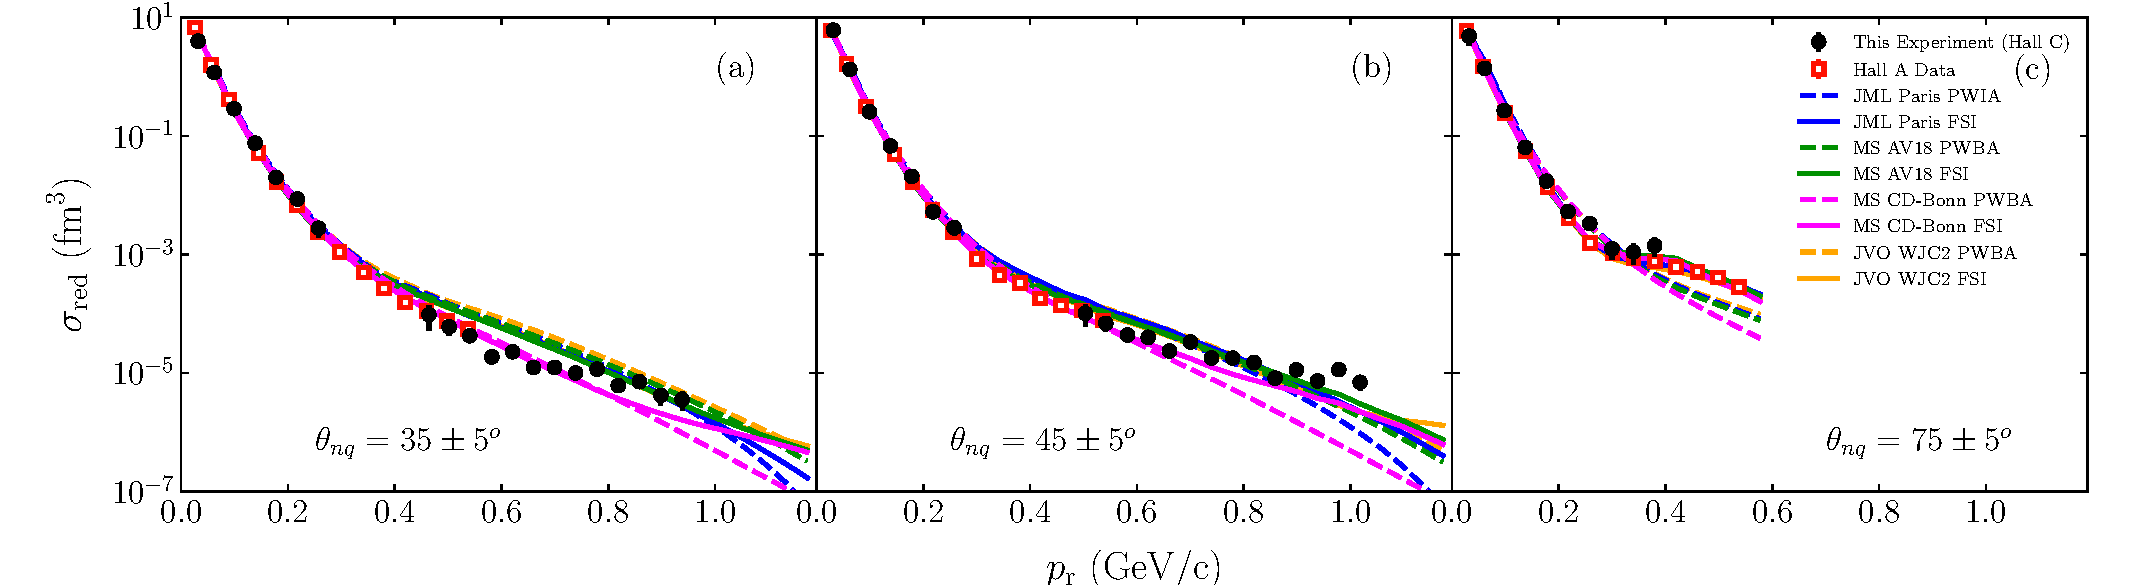
\includegraphics[scale=0.45]{PRL_plot1.pdf}
\caption{(Color online). The reduced cross sections $\sigma_{\mathrm{red}}(p_{\mathrm{r}})$ as a function of neutron recoil momentum $p_{\mathrm{r}}$ are shown in (a)-(c) for recoil angles $\theta_{nq}=35^{\circ}, 45^{\circ}$ and $75^{\circ}$, respectively,
with a bin width of $\pm 5^{\circ}$. The data are compared to the previous Hall A experiment (red square) results \cite{PhysRevLett.107.262501} as well as the theoretical reduced cross sections using the Paris (blue),
AV18 (green), CD-Bonn (magenta) and WJC2 (orange) $NN$ potentials.}
\label{fig:fig1}
\end{figure*}
\indent The data were radiatively corrected for each bin in ($\theta_{nq}, p_{\mathrm{r}}$) by multiplying the measured cross sections by the ratio of the calculated particle yield excluding and including radiative effects.
The SIMC simulation code was used for these calculations with the Deuteron Model by Laget including FSI \cite{LAGET2005}.
For each bin in ($\theta_{nq}, p_{\mathrm{r}}$), the averaged $^{2}\mathrm{H}(e,e'p)n$ kinematics was calculated and used in the bin centering correction factor defined as:
$f_{\mathrm{bc}} \equiv \sigma_{\mathrm{avg.kin}} / \bar{\sigma}$, where $\sigma_{\mathrm{avg.kin}}$ is the cross section calculated at the averaged kinematics and $\bar{\sigma}$ is the cross section averaged
over the kinematic bin. The systematic uncertainties associated with the radiative and bin-centering corrections were investigated using the Laget PWIA and FSI models but negligible effects
on the cross sections were found (see online Supplemental Material).
The experimental and theoretical reduced cross sections were extracted and are defined as follows:
\begin{equation}
\sigma_{\mathrm{red}} \equiv \frac{\sigma_{\mathrm{exp(th)}}}{E_{\mathrm{f}}p_{\mathrm{f}}f_{\mathrm{rec}}\sigma_{\mathrm{cc1}}},
\label{eq:1}
\end{equation}
\noindent where $\sigma_{\mathrm{exp(th)}}$ is the 5-fold experimental (or theoretical) differential cross section $\frac{d^{5}\sigma}{d\omega d\Omega_{e} d\Omega_{p}}$,
($E_{\mathrm{f}}, p_{\mathrm{f}}$) are the final proton energy and momentum, respectively, $f_{\mathrm{rec}}\equiv \frac{2p_{\mathrm{f}}^{2}E_{\mathrm{r}}}{2p_{\mathrm{f}}^{2}E_{\mathrm{r}} - (q^{2} - (p_{\mathrm{f}}^{2} + p_{\mathrm{r}}^{2}))E_{\mathrm{f}}}$
is a recoil factor obtained by integrating over the missing energy of the bound state in the 6-fold differential cross section where $E_{\mathrm{r}}$ is the neutron recoil energy, and $\sigma_{\mathrm{cc1}}$ is the
de Forest \cite{DEFOREST1983} electron-proton off-shell cross section calculated using the FF parametrization of Ref. \cite{PhysRevC.69.022201}.
Within the PWIA, $\sigma_{\mathrm{red}}$ corresponds to the PWIA cross section from the scattering of a proton in the deuteron. \\
\indent Figure \ref{fig:fig1} shows the extracted experimental and theoretical reduced cross sections as a function of $p_{\mathrm{r}}$ for three recoil angle settings at $Q^{2}=4.5\pm0.5$ (GeV/c)$^{2}$.
For the two highest momentum settings ($p_{\mathrm{r}}=580, 750$ MeV/c), a weighted average of the reduced cross sections were taken in the overlapping regions of $p_{\mathrm{r}}$. The results from the previous experiment \cite{PhysRevLett.107.262501} at a $Q^{2}=3.5\pm0.25$ (GeV/c)$^{2}$ are plotted as well (red square). %The good agreement between the Hall A and C data at lower $p_{\mathrm{r}}$ gives us confidence in the measurements made at higher missing momentum settings for which no previous data exist.
The data are compared to theoretical calculations using wave functions determined from the charge-dependent Bonn (CD-Bonn) \cite{PhysRevC.63.024001}, Argonne $v_{18}$ (AV18) \cite{PhysRevC.51.38}, Paris \cite{PhysRevC.21.861} and WJC2 \cite{Gross_2007} $NN$ potentials. The theoretical calculations
for the CD-Bonn (magenta) and AV18 (green) potentials were performed by Sargsian \cite{PhysRevC.82.014612} within the GEA, referred to as MS, and those for the Paris potential (blue) were by Laget \cite{LAGET2005} within the diagrammatic approach, referred to as JML.
For the WJC2 (orange) potential, the calculations were carried out by Ford, Jeschonnek and Van Orden \cite{PhysRevC.90.064006} using a Bethe-Salpeter-like formalism for two-body bound states, which will be labeled JVO.
The calculations use different FF parametrizations which can lead to a 6$\%$ change of the theortical cross section.\\
%----REMOVED ON 10/14/2020----------
%The MS calculations used the FF parametrization of Ref. \cite{PhysRevC.70.068202} while the JML calculations used the conventional dipole parametrization for
%the proton and neutron magnetic FF, the Galster \cite{Galster:1971} parametrization
%for the neutron electric FF, and the results from the Hall A experiment of Ref. \cite{PhysRevLett.88.092301} for the proton electric FF parametrization.
%The JVO calculations used two different FF parametrizations (GKex05 \cite{PhysRevC.66.045501}, AMT \cite{PhysRevC.76.035205}) where a
%difference of $\sim5.8-6.6 \%$ was found between the respective
%JVO reduced cross sections. Figure \ref{fig:fig1} shows the results using only the GKex05 parametrization. \\
\indent The difference between the deuteron wave functions with CD-Bonn, Paris, AV18 and WJC2 potentials is 
how the $NN$ potential is modeled based on the empirical $NN$ scattering data.
The CD-Bonn model is based on the One-Boson-Exchange Potential (OBEP) approach in which the 
nucleon-meson-meson couplings are constrained to describe the $NN$ scattering phase shifts
extracted from the data. The interaction potential represents the static limit of 
this potential. In contrast, the WJC2 is a OBEP derived within the Covariant Spectator Theory (CST) \cite{PhysRev.186.1448, PhysRevD.10.223, PhysRevC.26.2203, PhysRevC.26.2226}
which requires comparatively few parameters while still producing a high-precision fit to the $NN$ scattering data.
The Paris and AV18 are purely phenomenological potentials where a 
Yukawa type interaction is introduced and parameters are fitted to describe the 
same $NN$ scattering phase-shifts. The major difference between the CD-Bonn and Paris/AV18/WJC2 
potentials is that the former predicts a much softer repulsive interaction at short distance which 
results in a smaller high momentum component in the deuteron wave function in momentum space.
The effects of these local approximations on the $NN$ potential are shown in Fig. 2 of Ref. \cite{PhysRevC.63.024001}.\\
\indent For all recoil angles shown in Fig. \hyperref[fig:fig1]{1} at recoil momenta $p_{\mathrm{r}}\leq250$ MeV/c, the cross sections are well reproduced by all models when FSI are included.
The agreement at $p_{\mathrm{r}}\leq250$ MeV/c can be understood from the fact that this region corresponds to the long-range part of the $NN$ potential where the One Pion Exchange Potential (OPEP)
is well known and common to all modern potentials. \\
\indent Beyond $p_{\mathrm{r}}\sim250$ MeV/c at $\theta_{nq}=35^{\circ}$ and $45^{\circ}$ (Figs. \hyperref[fig:fig1]{1(a), 1(b)}), the JML,
MS AV18 and JVO models increasingly differ from the MS CD-Bonn calculation. In this region, the JML and MS AV18 cross sections are dominated by the PWIA and in good agreement up to $p_{\mathrm{r}}\sim700$ MeV/c whereas
the JVO PWIA falls off with a comparatively smaller cross section at $\theta_{nq}=35^{\circ}$. The MS CD-Bonn cross sections in contrast are generally smaller than the JML, MS AV18 and JVO in this region.
In addition, for $\theta_{nq}=35^{\circ}$, they are dominated by the PWIA up to $p_{\mathrm{r}}\sim800$ MeV/c
(Fig. \hyperref[fig:fig1]{1(a)}) while for $\theta_{nq}=45^{\circ}$ FSI start to contribute already above 600 MeV/c (Fig. \hyperref[fig:fig1]{1(b)}).\\
\indent For recoil momenta $p_{\mathrm{r}} \sim 0.55-1.0$ GeV/c (Figs. \hyperref[fig:fig1]{1(a), 1(b)}), all models exhibit a
steeper fall-off compared to data. This discrepancy was quantified by doing a linear fit to the data and each of the PWIA calculations. A difference of at least
4.2 standard deviations was found between the data and theory slopes which corresponds to a probability $\leq 1.1\times 10^{-5}$ (very unlikely) that the observed discrepancy is due to a statistical fluctuation. \\ 
\indent At $\theta_{nq}=75^{\circ}$ (Fig. \hyperref[fig:fig1]{1(c)}) and $p_{\mathrm{r}}>180$ MeV/c, FSI become the dominant contribution to the cross sections for all models which exhibit a similar
behavior (smaller fall-off) that overshadows any possibility of extracting the approximate momentum distributions.\\
\indent To quantify the discrepancy observed between data and theory in Fig. \ref{fig:fig1}, the ratio of the experimental and theoretical reduced cross sections ($\sigma_{\mathrm{red}}$) to the
deuteron momentum distribution calculated using the CD-Bonn potential ($\sigma^{\text{CD-Bonn PWIA}}_{\mathrm{red}}$) \cite{PhysRevC.63.024001} is shown in Fig. \ref{fig:fig2}. \\
\indent For $\theta_{nq}=35^{\circ}$ and $45^{\circ}$ (Figs. \hyperref[fig:fig2]{2(a),(b)}), the data are best described by the MS CD-Bonn PWIA calculation for recoil momenta up
to $p_{\mathrm{r}}\sim700$ MeV/c and $\sim600$ MeV/c, respectively. Furthermore, the agreement between the Halls A and C data validates the Hall A approach of selecting a kinematic
region where recoil angles are small and FSI are reduced. \\
\indent At larger recoil momenta, where the ratio $R>1$ and increasing with $p_{\mathrm{r}}$, for $\theta_{nq}=35^{\circ}$ FSI start to dominate at
$p_{\mathrm{r}} \gtrsim 800$ MeV/c for the MS CD-Bonn
\begin{figure}[!t]
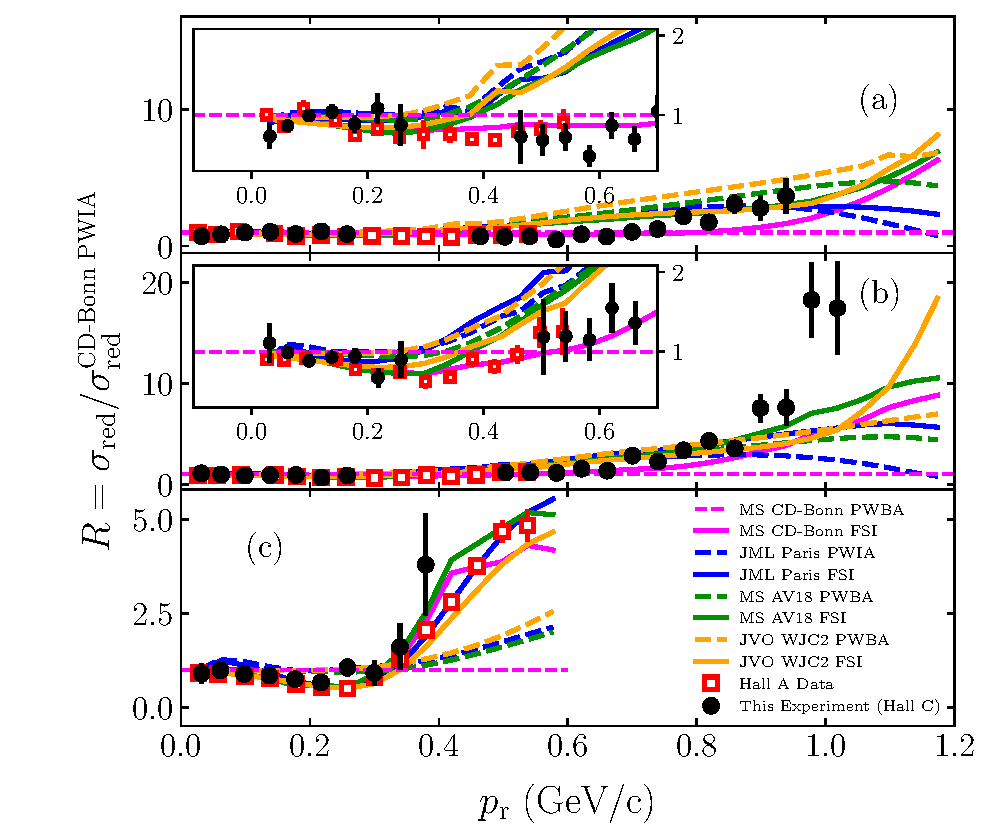
\includegraphics[scale=0.5]{PRL_plot2.pdf}
\caption{(Color online). The ratio $R(p_{\mathrm{r}}$) is shown in (a)-(c) for $\theta_{nq}=35^{\circ}, 45^{\circ}$ and $75^{\circ}$, respectively, each with a bin width of $\pm 5^{\circ}$.
  The dashed reference (magenta) line refers to MS CD-Bonn PWIA calculation (or momentum distribution) by which the data and all models are divided.
  Insets: Blowup of the subfigures below $p_{\mathrm{r}}=$0.7 GeV/c.}
\label{fig:fig2}
\end{figure}
calculation while the other models predict still relatively small FSI below 900 MeV/c.
At $\theta_{nq}=45^{\circ}$, the FSI dominance starts earlier for all models above 800 MeV/c and for the MS CD-Bonn based calculation above 600 MeV/c. \\
\indent Overall, it is interesting to note that none of the calculations can reproduce the measured $p_{\mathrm{r}}$ dependence above 600 MeV/c in a
region where FSI are still relatively small $(<30\%)$. This behavior of the data is new and additional data in this kinematic region are necessary
to improve the statistics. \\
\indent At $\theta_{nq}=75^{\circ}$ (Fig. \hyperref[fig:fig2]{2(c)}), FSI are small below $p_{\mathrm{r}}\sim180$ MeV/c, but do not exactly cancel the PWIA/FSI interference term in the scattering amplitude which results in a small dip in this region in agreement with the data.
At $p_{\mathrm{r}}>300$ MeV/c ($\theta_{nq}=75^{\circ}$), the data were statistically limited as our focus was on the smaller recoil angles. The Hall A data, however, show a reasonable agreement with the FSI from all models
which gives us confidence in our understanding of FSI at the smaller recoil angles. \\
\indent To summarize, this experiment extended the previous Hall A cross section measurements on the $^{2}\mathrm{H}(e,e'p)n$ reaction to 
$p_{\mathrm{r}}>500$ MeV/c at kinematics where FSI were expected to be small and the cross sections were dominated by PWIA and sensitive to the
short range part of the deuteron wave function. The experimental reduced cross sections were extracted and found to be in good agreement with the Hall A data at lower recoil momenta where they overlap.
Furthermore, the MS CD-Bonn model was found to be significantly different than the JML, MS AV18 or JVO models and was able to partially describe the data over a larger range in $p_{\mathrm{r}}$.
At the higher missing momenta provided by this experiment ($p_{\mathrm{r}}>700$ MeV/c), however, all models were unable to describe the data. 
Additional measurements of the $^{2}\mathrm{H}(e,e'p)n$ would be required to reduce the statistical uncertainties in this very high missing
momentum region ($p_{\mathrm{r}}>500$ MeV/c) to better understand the large deviations observed between the different models and data.\\
\indent We acknowledge the outstanding support of the staff of the Accelerator and Physics Divisions at Jefferson Lab
as well as the entire Hall C staff, technicians, graduate students and users who took shifts or contributed
to the equipment for the Hall C upgrade, making all four commissioning experiments possible. We would also like to
thank Misak Sargsian, J.M. Laget, Sabine Jeschonnek and J.W. Van Orden for providing the theoretical calculations as well as the useful
discussions we had on this topic. This work was supported in part by the U.S. Department of Energy (DOE), Office of Science, Office of Nuclear Physics
under grant No. DE-SC0013620 and contract DE-AC05-06OR23177, the Nuclear Regulatory Commission (NRC) Fellowship
under grant No. NRC-HQ-84-14-G-0040, the Doctoral Evidence Acquisition (DEA) Fellowship and the Natural Sciences and Engineering Research Council of Canada (NSERC).


%---include references that are not mentioned in the main text
%---but are included in the supplemental material
%---cite supp. material as follows:  (See Supplemental Material) after description of the topic being discussed.
%\nocite{COSY}
\nocite{barlow2002systematic}
\nocite{barlow2017}

\bibliography{ms}
\end{document}
